\subsection{Server Architecture}
\label{sec:server}

The server is structured in three layers: a dispatcher service, a logic layer and a data layer. This is based on the MVC Model described in \Cref{sec:mvc}. Because we wanted to develop a framework for creating location-based games, we had to make a decision how to achieve this goal. We could not interleave framework-specific functionality with the specific game we developed alongside our framework. Our solution was to create these three layers. We wanted to build a communication layer to handle the communication between the client and the server and a data layer to handle the communication between the server and the database. These two layers were chosen early in the design process. Our next choice was how to implement a specific game capable of using the framework, while still being scalable and encapsulated. We decided to make the threaded class called Game Thread handle all game-specific calculations, logics and responses. 
It was helpful to build a game alongside the framework. For example, this helped us to figure out the need for a service to handle timed events in the framework, which resulted in the Event Timer. We also discovered the need of a way to handle client requests that requested functionality prior to the Game Thread. This was requests like logging in, and seeing all active games, which cannot be handled by a game thread yet since it might not have been created yet. The result was the Admin. The Event Timer and the Admin are both positioned in the Logic Layer, because they help make logic decisions based on requests made by the client. 

%Server Architecture
\paragraph{Dispatcher Service}
The dispatcher is a service responsible for handling the communication with the client. It consists of an asynchronous I/O\fixme{IO or I/O throughout report?} and the dispatcher itself. Communication is done by an XML interface where requests from the client is verified by the dispatcher and passed to either the Admin module or a Game Thread depending on the message. 

\paragraph{Logic Layer}
This layer represents the business logic of the server application. The Admin module handles user creation, user login and game creation and is general for all game implementations. Game Thread is where specific game logic is implemented and its implementation will vary depending on the type of game. Event Timer is a general module handling events specified to happen at certain times. The game threads are responsible for creating events for themselves. The event timer will then notify a game thread at the specified time. As illustrated in \cref{fig:serverarch}, game threads are not a part of the framework, but can be ``plugged in''\fixme{change word??} to the framework. This increases the versatility of the game threads, since a developer can create his own game threads and plug them into the framework.

\paragraph{Data Layer}
Is the database representation in the model using the data mapper pattern\fxwarning{WE book ref}. The gateway is responsible for querying and updating the database and mapping the tables to objects used in the game logic and administration.

\begin{figure}[H]
  \centering
  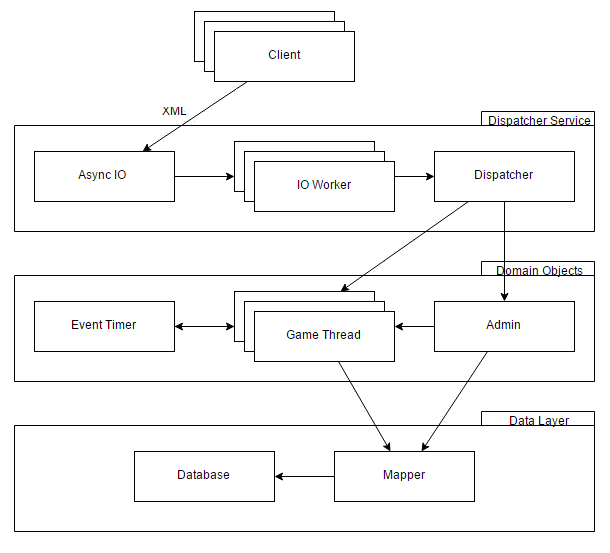
\includegraphics[width=\textwidth]{billeder/serverarch.png}  
  \caption{Architecture of server displaying the branching of an incoming connection}
  \label{fig:serverarch}
\end{figure}

%Dispatcher Service
\subsection{Dispatcher Service}
This layer is responsible for communication between client and server, this responsibility is divided between an IO module and a Dispatcher. In this section we will first examine Synchronous and Asynchronous IO in order to determine which is best suited for this framework and then the Dispatcher which forwards messages to the Logic Layer. 

The Asynchronous IO unit handles socket creation and TCP/IP communication, a rather trivial part of a client-server interface. The need for the Dispatcher unit was discovered by building our game. We need a way to dispatch requests from the client to the right component and method on the server. We dispatch to either Admin or Game Thread, by reading the request from the client and determine what type of request it is and continue accordingly. We decided to build the Dispatcher to encapsulate reading and analysing the requests from the client. Alternatively, we could have passed everything to Admin and incorporated the Dispatcher's functionality into the Admin, but we did not consider this a well structured framework.

% ms-syn-asyn - http://msdn.microsoft.com/en-us/library/windows/desktop/aa365683(v=vs.85).aspx


\section{Synchronous vs. Asynchronous I/O}
%What is B/NB I/O?
I/O can be handled either synchronously or asynchronously. A synchronous I/O operation is blocking, i.e., the thread that executes the current job is in a waiting state, where it does not compute anything, until it gets a response. An asynchronous I/O operation is non-blocking and therefore allows the thread to execute another job while waiting for the I/O operation to finish. This is illustrated on \Cref{fig:syncasync}. The figure does not show the overhead caused by using asynchronous I/O, which causes this to not always be the best solution, especially if there are many short I/O operations \cite{ms-syn-asyn}.

\begin{figure}[H]
  \centering
  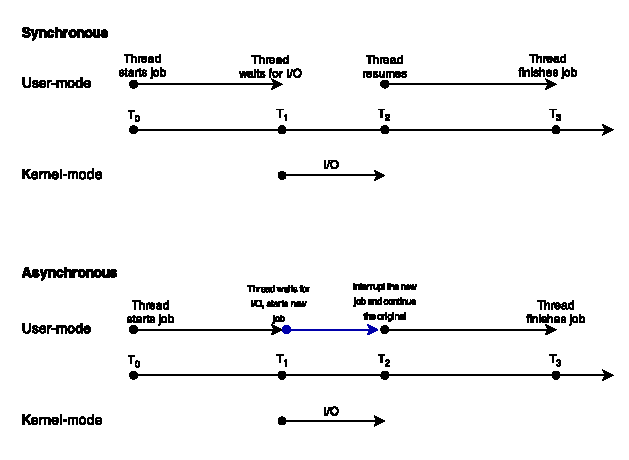
\includegraphics[scale=1.2]{billeder/sync-async.pdf}  
  \caption{Synchronous and asyncronous execution. Based on \cite{ms-syn-asyn}.}
  \label{fig:syncasync}
\end{figure}

This is the case for one or few users, but if there are many users at once they either have to wait in queue for previous I/O operations to finish, or each operation has to be executed in it's own thread, which would potentially result in many active threads, requiring a lot of memory. As pointed out by \citet{amir} it is worth noting that an asynchronous call that results in a synchronous operation causes the application to block, and therefore should be considered during implementation.

To enable the server to scale better, the I/O is implemented asynchronously. When the server receives an input, it is asynchronously sent to a dispatcher which sends it to the correct place; this is described in \Cref{sec:server}. Because of the many parts that have to interact, it is hard to determine if this implementation behaves as expected without testing it, but changing to a synchronous implementation would not be very expensive, as the asynchronous code is very similar to the synchronous code thanks to .NET's \texttt{Async} and \texttt{Await} keywords \cite{ms-asyn}. Making both implementations available at the same time, and letting the user choose which one to use, would also be relatively easy to do, but it adds some extra complexity to the code, as changes in one implementation would require similar changes in the other.
%What are the advantages and disadvantages?

%Which alternative(s) is/are there?

%Why did we make the choice we did?

%How flexible is it?
% - Could it easily be changed? 
% - Could both be implemented and the framework-user decides which one to use?
%
%\section{Synchronous vs. Asynchronous I/O}\fxfatal{This section will be rewritten with proper sources.}
%For the client/server socket communication, a choice between synchronous and asynchronous I/O has to be taken.
%% % blocking % %
%Synchronous I/O can have a better performance than asynchronous, but can cause problems when using a threaded architecture that spawns a new thread for each client. This is particularly true when the server should be scalable in regards to its number of connected clients. There might be 5 and there might be 5000 or even more.
%Tests show that threads are very efficient when it comes to memory and context switching, but only when the threads are kept alive for the entire execution of an application. This is not the case for our application, which will likely have many connections of varying durations during its up-time. \fixme{cite}\\\\
%% % non-blocking % %
%Asynchronous I/O is chosen for this project. It scales well when there are many clients, and the system should scale well with a potentially large number of clients. A notable advantage of asynchronous is that it limits the number of concurrent threads. The server asynchronously accepts a connection request from a client, and then starts an asynchronous worker thread to handle communication with the client. Meanwhile it continues to listen for new client connections.
%

%The ability to scale well does not come for free, however. Non-blocking IO is not always as fast as blocking IO and this can result in decreased performance. 
\subsection{Dispatcher}\label{subsec:dispatcherdesign}
The Dispatcher is a central component in the framework. It is placed in the \textit{Dispatcher Service} in the architecture, and is the first receiving to interpret a request sent by a client. The dispatcher simply dispatches a call to the appropriate method with the appropriate parameters when it receives XML data. In order to do this, it reads as little XML as possible to extract information to decide the appropriate destination and the right method to call. It attaches the entire XML as parameter to the method call.

The Dispatcher looks for the specified method call in the XML to hand it over to the Admin class. This is static calling of methods with attached XML. The Dispatcher waits for the Admin to return an XML, which it returns to the Async IO.

The Dispatcher handles all requests to a game thread dynamically, as it only interpret the method call before handing it over to the game thread. It then waits until the game thread returns a XML string, which it returns to the Async IO.

%Logic Layer
\subsection{Logic Layer}
This layer parses and reacts to the messages received from the Dispatcher. The logic layer interact with the Game Threads and consists of the Event Timer module which is callable from the Game Threads and can do a callback at a later time. The layer also contains the Admin module responsible for creating Game threads as well as non-game specifics such as authenticating logins.

The framework allows the user to use services like logging a client in through an XML-based interface. Services in the framework requires the user to implement proper XML-based communication on the client-side. A discussion about the use of XML seen in \ref{subsec:interfaces}. The framework also offers to handle Game Events, timed to occur after a specified time-stamp. This service used by creating a Game Event in the Game Thread being build by the user of the framework. We decided to build the Event Timer this way to encapsulate time-handling, and make a generic module that can be used for many different events. The user of the framework can specify what should happen for a given event in the Game Event class.

\subsubsection{Admin}\label{subsec:admindesign}
The Admin module is responsible for handling server-requests not related to specifict Game Threads. The Admin module handles administrative calls like creating new games or accounts as well as verifying login requests. 

%impl?
%A \textit{CreateGame} call cannot be send to a game thread, obviously because the game thread has not yet been created. Therefore this method will create a game from a model-class \textit{Game}, store it in the database with the provided settings, start a thread on the server for it to run on. 


\subsection{Event Timer}\label{subsec:eventtimerdesign}


%Game Block
\subsection{Game Block}
This is the workstation of the user of the framework. This block interacts with all the layers in the framework and makes use of the functionality provided by the framework. This class encapsulates all game-specific logic.

This is where we designed the framework to allow the user to develop a game. The framework has several rules the user has to follow when using the framework. They are explained for each module in the design. An example is the XML communication from client to server.
 
\subsection{Game thread-pool}
The game thread-pool is a collection of active game thread-instances, uniquely identified by a game-Id.

The game thread-pool is used as a handle to the game threads, and allows dynamic call to the desired game through method-parametrization. 

\subsection{Game thread}
\paragraph{Starting a game}
A game thread will be initialised and started when a user requests to host a game. A game will be assigned a game-id by the server, user-specified settings for hosting the game will be initialised and the game will be created in the database. 

When the server initialises each setting, it calls a method within the game thread-class. These methods calls the database-controller to change the state of the game in the database. These settings are:
\begin{itemize}
\item Game-privacy (Public or private game)
\item Number of teams
\item Game start-time
\item Game end-time
\item Game-boundary NorthWest GPS-coordinate
\item Game-boundary SouthEast GPS-coordinate
\end{itemize}

\paragraph{Updating a game}
Updates to a game can be split into two groups. One group is specific changes to a game, like inviting a new player or firing a gun. Another group is updating a players position when moving around in the game.

Updating a players position is trivial. The game thread receives a game-id, player-id and a new position. It calls the database-controller to store the new position in the database.

When performing an action like firing a gun, the server will have to fetch the gunman's position and the victim's position. It will then calculate if the range of the fired weapon allows the victim to be hit. If the shot is successful it will return that to the player, if the shot is unsuccessful it will return that the victim is out of range. 

All updates to change the state of a game will be in the game thread-class. This class will need to contain methods for all the in-game functionality. 

\paragraph{Closing a game}
When a game ends, the call will come from the timer thread. This will ask the game thread to clean up what is has stored in the database, and return a status message. The timer thread will then continue to close the game thread. 

%Data Layer
\subsection{Data Layer}
The data layer provides the user of the framework with the functionality to store data for later use. It is developed in a location-based game-format, as it was developed alongside our game.

\subsection{Database}\label{subsec:databasedesign}
\begin{figure}[H]
  \centering
  \includegraphics[width=\textwidth]{billeder/Server.tex}  
  \caption{Architecture of server displaying the branching of an incoming connection}
  \label{fig:serverarchitecture}
\end{figure}
In this project a database was needed to keep track of all information related to users and games they are playing. The database is designed with flexibility in mind which means that the logic behind a game is responsible for interpreting the data in the database. \figref{fig:ER}\fxwarning{export new ER diagram} shows the entity relation diagram for the database without attributes. The database is structured as follows:

\begin{figure}
  \centering
  % Graphic for TeX using PGF
% \usepackage{tikz}
% The following commands are not supported in PSTricks at present
% We define them conditionally, so when they are implemented,
% this pgf file will use them.
\ifx\du\undefined
  \newlength{\du}
\fi
\setlength{\du}{15\unitlength}
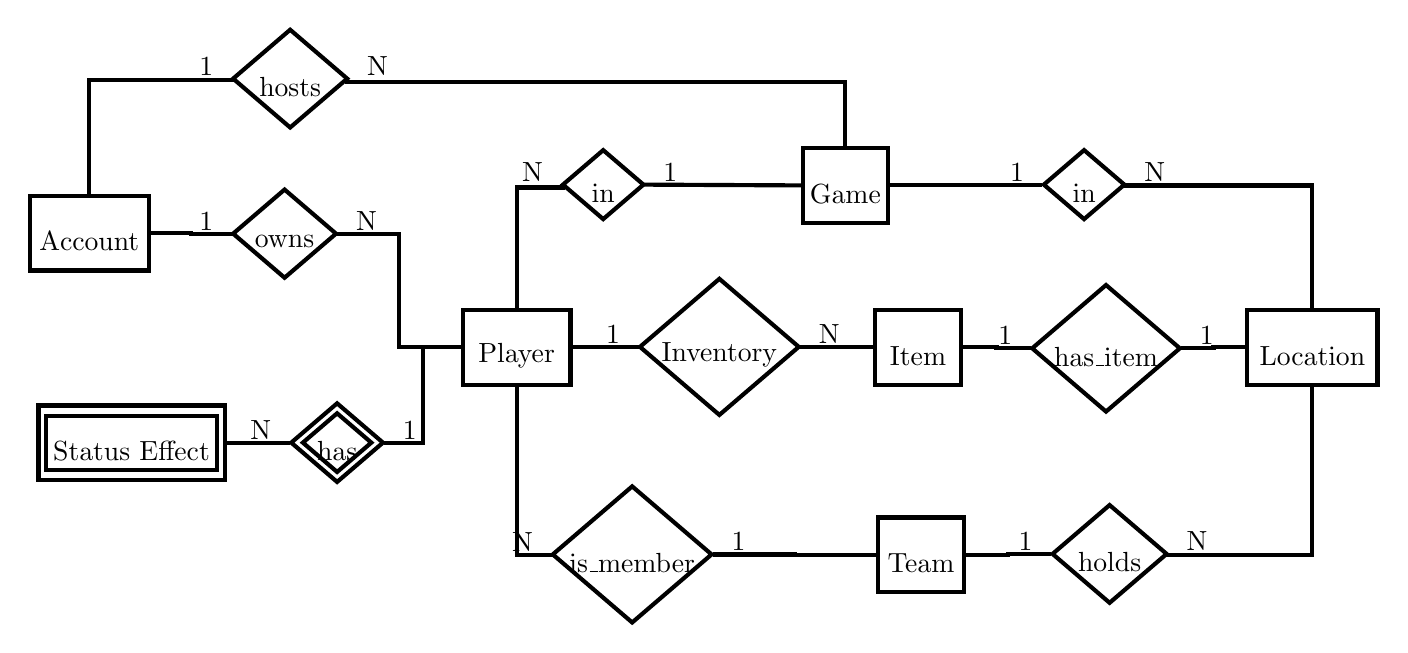
\begin{tikzpicture}
\pgftransformxscale{0.700000}
\pgftransformyscale{-1.000000}
\definecolor{dialinecolor}{rgb}{0.000000, 0.000000, 0.000000}
\pgfsetstrokecolor{dialinecolor}
\definecolor{dialinecolor}{rgb}{1.000000, 1.000000, 1.000000}
\pgfsetfillcolor{dialinecolor}
\definecolor{dialinecolor}{rgb}{1.000000, 1.000000, 1.000000}
\pgfsetfillcolor{dialinecolor}
\fill (-8.000000\du,-6.000000\du)--(-8.000000\du,-4.200000\du)--(-3.905000\du,-4.200000\du)--(-3.905000\du,-6.000000\du)--cycle;
\pgfsetlinewidth{0.100000\du}
\pgfsetdash{}{0pt}
\pgfsetmiterjoin
\definecolor{dialinecolor}{rgb}{0.000000, 0.000000, 0.000000}
\pgfsetstrokecolor{dialinecolor}
\draw (-8.000000\du,-6.000000\du)--(-8.000000\du,-4.200000\du)--(-3.905000\du,-4.200000\du)--(-3.905000\du,-6.000000\du)--cycle;
% setfont left to latex
\definecolor{dialinecolor}{rgb}{0.000000, 0.000000, 0.000000}
\pgfsetstrokecolor{dialinecolor}
\node at (-5.952500\du,-4.900000\du){Account};
\definecolor{dialinecolor}{rgb}{1.000000, 1.000000, 1.000000}
\pgfsetfillcolor{dialinecolor}
\fill (18.600000\du,-7.150000\du)--(18.600000\du,-5.350000\du)--(21.540000\du,-5.350000\du)--(21.540000\du,-7.150000\du)--cycle;
\pgfsetlinewidth{0.100000\du}
\pgfsetdash{}{0pt}
\pgfsetmiterjoin
\definecolor{dialinecolor}{rgb}{0.000000, 0.000000, 0.000000}
\pgfsetstrokecolor{dialinecolor}
\draw (18.600000\du,-7.150000\du)--(18.600000\du,-5.350000\du)--(21.540000\du,-5.350000\du)--(21.540000\du,-7.150000\du)--cycle;
% setfont left to latex
\definecolor{dialinecolor}{rgb}{0.000000, 0.000000, 0.000000}
\pgfsetstrokecolor{dialinecolor}
\node at (20.070000\du,-6.050000\du){Game};
\definecolor{dialinecolor}{rgb}{1.000000, 1.000000, 1.000000}
\pgfsetfillcolor{dialinecolor}
\fill (21.200000\du,1.750000\du)--(21.200000\du,3.550000\du)--(24.140000\du,3.550000\du)--(24.140000\du,1.750000\du)--cycle;
\pgfsetlinewidth{0.100000\du}
\pgfsetdash{}{0pt}
\pgfsetmiterjoin
\definecolor{dialinecolor}{rgb}{0.000000, 0.000000, 0.000000}
\pgfsetstrokecolor{dialinecolor}
\draw (21.200000\du,1.750000\du)--(21.200000\du,3.550000\du)--(24.140000\du,3.550000\du)--(24.140000\du,1.750000\du)--cycle;
% setfont left to latex
\definecolor{dialinecolor}{rgb}{0.000000, 0.000000, 0.000000}
\pgfsetstrokecolor{dialinecolor}
\node at (22.670000\du,2.850000\du){Team};
% setfont left to latex
\definecolor{dialinecolor}{rgb}{0.000000, 0.000000, 0.000000}
\pgfsetstrokecolor{dialinecolor}
\node[anchor=west] at (22.670000\du,2.650000\du){};
\definecolor{dialinecolor}{rgb}{1.000000, 1.000000, 1.000000}
\pgfsetfillcolor{dialinecolor}
\fill (13.000000\du,-2.360500\du)--(15.732500\du,-4.000000\du)--(18.465000\du,-2.360500\du)--(15.732500\du,-0.721000\du)--cycle;
\pgfsetlinewidth{0.100000\du}
\pgfsetdash{}{0pt}
\pgfsetmiterjoin
\definecolor{dialinecolor}{rgb}{0.000000, 0.000000, 0.000000}
\pgfsetstrokecolor{dialinecolor}
\draw (13.000000\du,-2.360500\du)--(15.732500\du,-4.000000\du)--(18.465000\du,-2.360500\du)--(15.732500\du,-0.721000\du)--cycle;
% setfont left to latex
\definecolor{dialinecolor}{rgb}{0.000000, 0.000000, 0.000000}
\pgfsetstrokecolor{dialinecolor}
\node[anchor=east] at (12.700000\du,-2.660500\du){1};
\definecolor{dialinecolor}{rgb}{0.000000, 0.000000, 0.000000}
\pgfsetstrokecolor{dialinecolor}
\node[anchor=west] at (18.765000\du,-2.660500\du){N};
\definecolor{dialinecolor}{rgb}{0.000000, 0.000000, 0.000000}
\pgfsetstrokecolor{dialinecolor}
\node at (15.732500\du,-2.160500\du){Inventory};
\definecolor{dialinecolor}{rgb}{1.000000, 1.000000, 1.000000}
\pgfsetfillcolor{dialinecolor}
\fill (21.100000\du,-3.250000\du)--(21.100000\du,-1.450000\du)--(24.040000\du,-1.450000\du)--(24.040000\du,-3.250000\du)--cycle;
\pgfsetlinewidth{0.100000\du}
\pgfsetdash{}{0pt}
\pgfsetmiterjoin
\definecolor{dialinecolor}{rgb}{0.000000, 0.000000, 0.000000}
\pgfsetstrokecolor{dialinecolor}
\draw (21.100000\du,-3.250000\du)--(21.100000\du,-1.450000\du)--(24.040000\du,-1.450000\du)--(24.040000\du,-3.250000\du)--cycle;
% setfont left to latex
\definecolor{dialinecolor}{rgb}{0.000000, 0.000000, 0.000000}
\pgfsetstrokecolor{dialinecolor}
\node at (22.570000\du,-2.150000\du){Item};
\definecolor{dialinecolor}{rgb}{1.000000, 1.000000, 1.000000}
\pgfsetfillcolor{dialinecolor}
\fill (26.500000\du,-2.325999\du)--(29.040000\du,-3.849999\du)--(31.580000\du,-2.325999\du)--(29.040000\du,-0.801999\du)--cycle;
\pgfsetlinewidth{0.100000\du}
\pgfsetdash{}{0pt}
\pgfsetmiterjoin
\definecolor{dialinecolor}{rgb}{0.000000, 0.000000, 0.000000}
\pgfsetstrokecolor{dialinecolor}
\draw (26.500000\du,-2.325999\du)--(29.040000\du,-3.849999\du)--(31.580000\du,-2.325999\du)--(29.040000\du,-0.801999\du)--cycle;
% setfont left to latex
\definecolor{dialinecolor}{rgb}{0.000000, 0.000000, 0.000000}
\pgfsetstrokecolor{dialinecolor}
\node[anchor=east] at (26.200000\du,-2.625999\du){1};
\definecolor{dialinecolor}{rgb}{0.000000, 0.000000, 0.000000}
\pgfsetstrokecolor{dialinecolor}
\node[anchor=west] at (31.880000\du,-2.625999\du){1};
\definecolor{dialinecolor}{rgb}{0.000000, 0.000000, 0.000000}
\pgfsetstrokecolor{dialinecolor}
\node at (29.040000\du,-2.125999\du){has\_item};
\definecolor{dialinecolor}{rgb}{1.000000, 1.000000, 1.000000}
\pgfsetfillcolor{dialinecolor}
\fill (33.900000\du,-3.250000\du)--(33.900000\du,-1.450000\du)--(38.380000\du,-1.450000\du)--(38.380000\du,-3.250000\du)--cycle;
\pgfsetlinewidth{0.100000\du}
\pgfsetdash{}{0pt}
\pgfsetmiterjoin
\definecolor{dialinecolor}{rgb}{0.000000, 0.000000, 0.000000}
\pgfsetstrokecolor{dialinecolor}
\draw (33.900000\du,-3.250000\du)--(33.900000\du,-1.450000\du)--(38.380000\du,-1.450000\du)--(38.380000\du,-3.250000\du)--cycle;
% setfont left to latex
\definecolor{dialinecolor}{rgb}{0.000000, 0.000000, 0.000000}
\pgfsetstrokecolor{dialinecolor}
\node at (36.140000\du,-2.150000\du){Location};
\definecolor{dialinecolor}{rgb}{1.000000, 1.000000, 1.000000}
\pgfsetfillcolor{dialinecolor}
\fill (27.200004\du,2.627500\du)--(29.162504\du,1.450000\du)--(31.125004\du,2.627500\du)--(29.162504\du,3.805000\du)--cycle;
\pgfsetlinewidth{0.100000\du}
\pgfsetdash{}{0pt}
\pgfsetmiterjoin
\definecolor{dialinecolor}{rgb}{0.000000, 0.000000, 0.000000}
\pgfsetstrokecolor{dialinecolor}
\draw (27.200004\du,2.627500\du)--(29.162504\du,1.450000\du)--(31.125004\du,2.627500\du)--(29.162504\du,3.805000\du)--cycle;
% setfont left to latex
\definecolor{dialinecolor}{rgb}{0.000000, 0.000000, 0.000000}
\pgfsetstrokecolor{dialinecolor}
\node[anchor=east] at (26.900004\du,2.327500\du){1};
\definecolor{dialinecolor}{rgb}{0.000000, 0.000000, 0.000000}
\pgfsetstrokecolor{dialinecolor}
\node[anchor=west] at (31.425004\du,2.327500\du){N};
\definecolor{dialinecolor}{rgb}{0.000000, 0.000000, 0.000000}
\pgfsetstrokecolor{dialinecolor}
\node at (29.162504\du,2.827500\du){holds};
\definecolor{dialinecolor}{rgb}{1.000000, 1.000000, 1.000000}
\pgfsetfillcolor{dialinecolor}
\fill (26.900004\du,-6.268999\du)--(28.285004\du,-7.099999\du)--(29.670004\du,-6.268999\du)--(28.285004\du,-5.437999\du)--cycle;
\pgfsetlinewidth{0.100000\du}
\pgfsetdash{}{0pt}
\pgfsetmiterjoin
\definecolor{dialinecolor}{rgb}{0.000000, 0.000000, 0.000000}
\pgfsetstrokecolor{dialinecolor}
\draw (26.900004\du,-6.268999\du)--(28.285004\du,-7.099999\du)--(29.670004\du,-6.268999\du)--(28.285004\du,-5.437999\du)--cycle;
% setfont left to latex
\definecolor{dialinecolor}{rgb}{0.000000, 0.000000, 0.000000}
\pgfsetstrokecolor{dialinecolor}
\node[anchor=east] at (26.600004\du,-6.568999\du){1};
\definecolor{dialinecolor}{rgb}{0.000000, 0.000000, 0.000000}
\pgfsetstrokecolor{dialinecolor}
\node[anchor=west] at (29.970004\du,-6.568999\du){N};
\definecolor{dialinecolor}{rgb}{0.000000, 0.000000, 0.000000}
\pgfsetstrokecolor{dialinecolor}
\node at (28.285004\du,-6.068999\du){in};
\definecolor{dialinecolor}{rgb}{1.000000, 1.000000, 1.000000}
\pgfsetfillcolor{dialinecolor}
\fill (-1.000000\du,-8.822500\du)--(0.962500\du,-10.000000\du)--(2.925000\du,-8.822500\du)--(0.962500\du,-7.645000\du)--cycle;
\pgfsetlinewidth{0.100000\du}
\pgfsetdash{}{0pt}
\pgfsetmiterjoin
\definecolor{dialinecolor}{rgb}{0.000000, 0.000000, 0.000000}
\pgfsetstrokecolor{dialinecolor}
\draw (-1.000000\du,-8.822500\du)--(0.962500\du,-10.000000\du)--(2.925000\du,-8.822500\du)--(0.962500\du,-7.645000\du)--cycle;
% setfont left to latex
\definecolor{dialinecolor}{rgb}{0.000000, 0.000000, 0.000000}
\pgfsetstrokecolor{dialinecolor}
\node[anchor=east] at (-1.300000\du,-9.122500\du){1};
\definecolor{dialinecolor}{rgb}{0.000000, 0.000000, 0.000000}
\pgfsetstrokecolor{dialinecolor}
\node[anchor=west] at (3.225000\du,-9.122500\du){N};
\definecolor{dialinecolor}{rgb}{0.000000, 0.000000, 0.000000}
\pgfsetstrokecolor{dialinecolor}
\node at (0.962500\du,-8.622500\du){hosts};
\definecolor{dialinecolor}{rgb}{1.000000, 1.000000, 1.000000}
\pgfsetfillcolor{dialinecolor}
\fill (6.900000\du,-3.250001\du)--(6.900000\du,-1.450001\du)--(10.610000\du,-1.450001\du)--(10.610000\du,-3.250001\du)--cycle;
\pgfsetlinewidth{0.100000\du}
\pgfsetdash{}{0pt}
\pgfsetmiterjoin
\definecolor{dialinecolor}{rgb}{0.000000, 0.000000, 0.000000}
\pgfsetstrokecolor{dialinecolor}
\draw (6.900000\du,-3.250001\du)--(6.900000\du,-1.450001\du)--(10.610000\du,-1.450001\du)--(10.610000\du,-3.250001\du)--cycle;
% setfont left to latex
\definecolor{dialinecolor}{rgb}{0.000000, 0.000000, 0.000000}
\pgfsetstrokecolor{dialinecolor}
\node at (8.755000\du,-2.150001\du){Player};
\definecolor{dialinecolor}{rgb}{1.000000, 1.000000, 1.000000}
\pgfsetfillcolor{dialinecolor}
\fill (-1.000000\du,-5.088000\du)--(0.770000\du,-6.150000\du)--(2.540000\du,-5.088000\du)--(0.770000\du,-4.026000\du)--cycle;
\pgfsetlinewidth{0.100000\du}
\pgfsetdash{}{0pt}
\pgfsetmiterjoin
\definecolor{dialinecolor}{rgb}{0.000000, 0.000000, 0.000000}
\pgfsetstrokecolor{dialinecolor}
\draw (-1.000000\du,-5.088000\du)--(0.770000\du,-6.150000\du)--(2.540000\du,-5.088000\du)--(0.770000\du,-4.026000\du)--cycle;
% setfont left to latex
\definecolor{dialinecolor}{rgb}{0.000000, 0.000000, 0.000000}
\pgfsetstrokecolor{dialinecolor}
\node[anchor=east] at (-1.300000\du,-5.388000\du){1};
\definecolor{dialinecolor}{rgb}{0.000000, 0.000000, 0.000000}
\pgfsetstrokecolor{dialinecolor}
\node[anchor=west] at (2.840000\du,-5.388000\du){N};
\definecolor{dialinecolor}{rgb}{0.000000, 0.000000, 0.000000}
\pgfsetstrokecolor{dialinecolor}
\node at (0.770000\du,-4.888000\du){owns};
\definecolor{dialinecolor}{rgb}{1.000000, 1.000000, 1.000000}
\pgfsetfillcolor{dialinecolor}
\fill (10.350000\du,-6.269000\du)--(11.735000\du,-7.100000\du)--(13.120000\du,-6.269000\du)--(11.735000\du,-5.438000\du)--cycle;
\pgfsetlinewidth{0.100000\du}
\pgfsetdash{}{0pt}
\pgfsetmiterjoin
\definecolor{dialinecolor}{rgb}{0.000000, 0.000000, 0.000000}
\pgfsetstrokecolor{dialinecolor}
\draw (10.350000\du,-6.269000\du)--(11.735000\du,-7.100000\du)--(13.120000\du,-6.269000\du)--(11.735000\du,-5.438000\du)--cycle;
% setfont left to latex
\definecolor{dialinecolor}{rgb}{0.000000, 0.000000, 0.000000}
\pgfsetstrokecolor{dialinecolor}
\node[anchor=east] at (10.050000\du,-6.569000\du){N};
\definecolor{dialinecolor}{rgb}{0.000000, 0.000000, 0.000000}
\pgfsetstrokecolor{dialinecolor}
\node[anchor=west] at (13.420000\du,-6.569000\du){1};
\definecolor{dialinecolor}{rgb}{0.000000, 0.000000, 0.000000}
\pgfsetstrokecolor{dialinecolor}
\node at (11.735000\du,-6.069000\du){in};
\pgfsetlinewidth{0.100000\du}
\pgfsetdash{}{0pt}
\pgfsetdash{}{0pt}
\pgfsetbuttcap
{
\definecolor{dialinecolor}{rgb}{0.000000, 0.000000, 0.000000}
\pgfsetfillcolor{dialinecolor}
% was here!!!
\definecolor{dialinecolor}{rgb}{0.000000, 0.000000, 0.000000}
\pgfsetstrokecolor{dialinecolor}
\draw (13.120000\du,-6.269000\du)--(18.600000\du,-6.250000\du);
}
\definecolor{dialinecolor}{rgb}{1.000000, 1.000000, 1.000000}
\pgfsetfillcolor{dialinecolor}
\fill (10.000000\du,2.639500\du)--(12.732500\du,1.000000\du)--(15.465000\du,2.639500\du)--(12.732500\du,4.279000\du)--cycle;
\pgfsetlinewidth{0.100000\du}
\pgfsetdash{}{0pt}
\pgfsetmiterjoin
\definecolor{dialinecolor}{rgb}{0.000000, 0.000000, 0.000000}
\pgfsetstrokecolor{dialinecolor}
\draw (10.000000\du,2.639500\du)--(12.732500\du,1.000000\du)--(15.465000\du,2.639500\du)--(12.732500\du,4.279000\du)--cycle;
% setfont left to latex
\definecolor{dialinecolor}{rgb}{0.000000, 0.000000, 0.000000}
\pgfsetstrokecolor{dialinecolor}
\node[anchor=east] at (9.700000\du,2.339500\du){N};
\definecolor{dialinecolor}{rgb}{0.000000, 0.000000, 0.000000}
\pgfsetstrokecolor{dialinecolor}
\node[anchor=west] at (15.765000\du,2.339500\du){1};
\definecolor{dialinecolor}{rgb}{0.000000, 0.000000, 0.000000}
\pgfsetstrokecolor{dialinecolor}
\node at (12.732500\du,2.839500\du){is\_member};
\definecolor{dialinecolor}{rgb}{1.000000, 1.000000, 1.000000}
\pgfsetfillcolor{dialinecolor}
\fill (-7.700000\du,-0.949999\du)--(-7.700000\du,0.850001\du)--(-1.295000\du,0.850001\du)--(-1.295000\du,-0.949999\du)--cycle;
\pgfsetlinewidth{0.100000\du}
\pgfsetdash{}{0pt}
\pgfsetmiterjoin
\definecolor{dialinecolor}{rgb}{0.000000, 0.000000, 0.000000}
\pgfsetstrokecolor{dialinecolor}
\draw (-7.700000\du,-0.949999\du)--(-7.700000\du,0.850001\du)--(-1.295000\du,0.850001\du)--(-1.295000\du,-0.949999\du)--cycle;
\definecolor{dialinecolor}{rgb}{0.000000, 0.000000, 0.000000}
\pgfsetstrokecolor{dialinecolor}
\draw (-7.450000\du,-0.699999\du)--(-7.450000\du,0.600001\du)--(-1.545000\du,0.600001\du)--(-1.545000\du,-0.699999\du)--cycle;
% setfont left to latex
\definecolor{dialinecolor}{rgb}{0.000000, 0.000000, 0.000000}
\pgfsetstrokecolor{dialinecolor}
\node at (-4.497500\du,0.150001\du){Status Effect};
\definecolor{dialinecolor}{rgb}{1.000000, 1.000000, 1.000000}
\pgfsetfillcolor{dialinecolor}
\fill (1.000000\du,-0.053500\du)--(2.577500\du,-1.000000\du)--(4.155000\du,-0.053500\du)--(2.577500\du,0.893000\du)--cycle;
\pgfsetlinewidth{0.100000\du}
\pgfsetdash{}{0pt}
\pgfsetmiterjoin
\definecolor{dialinecolor}{rgb}{0.000000, 0.000000, 0.000000}
\pgfsetstrokecolor{dialinecolor}
\draw (1.000000\du,-0.053500\du)--(2.577500\du,-1.000000\du)--(4.155000\du,-0.053500\du)--(2.577500\du,0.893000\du)--cycle;
\definecolor{dialinecolor}{rgb}{0.000000, 0.000000, 0.000000}
\pgfsetstrokecolor{dialinecolor}
\draw (1.400000\du,-0.053500\du)--(2.577500\du,-0.760000\du)--(3.755000\du,-0.053500\du)--(2.577500\du,0.653000\du)--cycle;
% setfont left to latex
\definecolor{dialinecolor}{rgb}{0.000000, 0.000000, 0.000000}
\pgfsetstrokecolor{dialinecolor}
\node[anchor=east] at (0.700000\du,-0.353500\du){N};
\definecolor{dialinecolor}{rgb}{0.000000, 0.000000, 0.000000}
\pgfsetstrokecolor{dialinecolor}
\node[anchor=west] at (4.455000\du,-0.353500\du){1};
\definecolor{dialinecolor}{rgb}{0.000000, 0.000000, 0.000000}
\pgfsetstrokecolor{dialinecolor}
\node at (2.577500\du,0.146500\du){has};
\pgfsetlinewidth{0.100000\du}
\pgfsetdash{}{0pt}
\pgfsetdash{}{0pt}
\pgfsetmiterjoin
\pgfsetbuttcap
{
\definecolor{dialinecolor}{rgb}{0.000000, 0.000000, 0.000000}
\pgfsetfillcolor{dialinecolor}
% was here!!!
{\pgfsetcornersarced{\pgfpoint{0.000000\du}{0.000000\du}}\definecolor{dialinecolor}{rgb}{0.000000, 0.000000, 0.000000}
\pgfsetstrokecolor{dialinecolor}
\draw (20.070000\du,-7.150000\du)--(20.070000\du,-8.749106\du)--(2.925000\du,-8.749106\du)--(2.925000\du,-8.822500\du);
}}
\pgfsetlinewidth{0.100000\du}
\pgfsetdash{}{0pt}
\pgfsetdash{}{0pt}
\pgfsetmiterjoin
\pgfsetbuttcap
{
\definecolor{dialinecolor}{rgb}{0.000000, 0.000000, 0.000000}
\pgfsetfillcolor{dialinecolor}
% was here!!!
{\pgfsetcornersarced{\pgfpoint{0.000000\du}{0.000000\du}}\definecolor{dialinecolor}{rgb}{0.000000, 0.000000, 0.000000}
\pgfsetstrokecolor{dialinecolor}
\draw (-1.000000\du,-8.822500\du)--(-1.000000\du,-8.799106\du)--(-5.952500\du,-8.799106\du)--(-5.952500\du,-6.000000\du);
}}
\pgfsetlinewidth{0.100000\du}
\pgfsetdash{}{0pt}
\pgfsetdash{}{0pt}
\pgfsetmiterjoin
\pgfsetbuttcap
{
\definecolor{dialinecolor}{rgb}{0.000000, 0.000000, 0.000000}
\pgfsetfillcolor{dialinecolor}
% was here!!!
{\pgfsetcornersarced{\pgfpoint{0.000000\du}{0.000000\du}}\definecolor{dialinecolor}{rgb}{0.000000, 0.000000, 0.000000}
\pgfsetstrokecolor{dialinecolor}
\draw (-1.000000\du,-5.088000\du)--(-2.452500\du,-5.088000\du)--(-2.452500\du,-5.100000\du)--(-3.905000\du,-5.100000\du);
}}
\pgfsetlinewidth{0.100000\du}
\pgfsetdash{}{0pt}
\pgfsetdash{}{0pt}
\pgfsetmiterjoin
\pgfsetbuttcap
{
\definecolor{dialinecolor}{rgb}{0.000000, 0.000000, 0.000000}
\pgfsetfillcolor{dialinecolor}
% was here!!!
{\pgfsetcornersarced{\pgfpoint{0.000000\du}{0.000000\du}}\definecolor{dialinecolor}{rgb}{0.000000, 0.000000, 0.000000}
\pgfsetstrokecolor{dialinecolor}
\draw (2.540000\du,-5.088000\du)--(4.720000\du,-5.088000\du)--(4.720000\du,-2.350001\du)--(6.900000\du,-2.350001\du);
}}
\pgfsetlinewidth{0.100000\du}
\pgfsetdash{}{0pt}
\pgfsetdash{}{0pt}
\pgfsetmiterjoin
\pgfsetbuttcap
{
\definecolor{dialinecolor}{rgb}{0.000000, 0.000000, 0.000000}
\pgfsetfillcolor{dialinecolor}
% was here!!!
{\pgfsetcornersarced{\pgfpoint{0.000000\du}{0.000000\du}}\definecolor{dialinecolor}{rgb}{0.000000, 0.000000, 0.000000}
\pgfsetstrokecolor{dialinecolor}
\draw (10.350000\du,-6.269000\du)--(10.350000\du,-6.199108\du)--(8.755000\du,-6.199108\du)--(8.755000\du,-3.299591\du);
}}
\pgfsetlinewidth{0.100000\du}
\pgfsetdash{}{0pt}
\pgfsetdash{}{0pt}
\pgfsetmiterjoin
\pgfsetbuttcap
{
\definecolor{dialinecolor}{rgb}{0.000000, 0.000000, 0.000000}
\pgfsetfillcolor{dialinecolor}
% was here!!!
{\pgfsetcornersarced{\pgfpoint{0.000000\du}{0.000000\du}}\definecolor{dialinecolor}{rgb}{0.000000, 0.000000, 0.000000}
\pgfsetstrokecolor{dialinecolor}
\draw (6.849535\du,-2.350001\du)--(5.527070\du,-2.350001\du)--(5.527070\du,-0.053500\du)--(4.204606\du,-0.053500\du);
}}
\pgfsetlinewidth{0.100000\du}
\pgfsetdash{}{0pt}
\pgfsetdash{}{0pt}
\pgfsetmiterjoin
\pgfsetbuttcap
{
\definecolor{dialinecolor}{rgb}{0.000000, 0.000000, 0.000000}
\pgfsetfillcolor{dialinecolor}
% was here!!!
{\pgfsetcornersarced{\pgfpoint{0.000000\du}{0.000000\du}}\definecolor{dialinecolor}{rgb}{0.000000, 0.000000, 0.000000}
\pgfsetstrokecolor{dialinecolor}
\draw (12.952405\du,-2.360500\du)--(11.806435\du,-2.360500\du)--(11.806435\du,-2.350001\du)--(10.660465\du,-2.350001\du);
}}
\pgfsetlinewidth{0.100000\du}
\pgfsetdash{}{0pt}
\pgfsetdash{}{0pt}
\pgfsetmiterjoin
\pgfsetbuttcap
{
\definecolor{dialinecolor}{rgb}{0.000000, 0.000000, 0.000000}
\pgfsetfillcolor{dialinecolor}
% was here!!!
{\pgfsetcornersarced{\pgfpoint{0.000000\du}{0.000000\du}}\definecolor{dialinecolor}{rgb}{0.000000, 0.000000, 0.000000}
\pgfsetstrokecolor{dialinecolor}
\draw (21.049629\du,-2.350000\du)--(19.781112\du,-2.350000\du)--(19.781112\du,-2.360500\du)--(18.512595\du,-2.360500\du);
}}
\pgfsetlinewidth{0.100000\du}
\pgfsetdash{}{0pt}
\pgfsetdash{}{0pt}
\pgfsetmiterjoin
\pgfsetbuttcap
{
\definecolor{dialinecolor}{rgb}{0.000000, 0.000000, 0.000000}
\pgfsetfillcolor{dialinecolor}
% was here!!!
{\pgfsetcornersarced{\pgfpoint{0.000000\du}{0.000000\du}}\definecolor{dialinecolor}{rgb}{0.000000, 0.000000, 0.000000}
\pgfsetstrokecolor{dialinecolor}
\draw (24.090371\du,-2.350000\du)--(25.271496\du,-2.350000\du)--(25.271496\du,-2.325999\du)--(26.452622\du,-2.325999\du);
}}
\pgfsetlinewidth{0.100000\du}
\pgfsetdash{}{0pt}
\pgfsetdash{}{0pt}
\pgfsetmiterjoin
\pgfsetbuttcap
{
\definecolor{dialinecolor}{rgb}{0.000000, 0.000000, 0.000000}
\pgfsetfillcolor{dialinecolor}
% was here!!!
{\pgfsetcornersarced{\pgfpoint{0.000000\du}{0.000000\du}}\definecolor{dialinecolor}{rgb}{0.000000, 0.000000, 0.000000}
\pgfsetstrokecolor{dialinecolor}
\draw (21.590371\du,-6.250000\du)--(24.220066\du,-6.250000\du)--(24.220066\du,-6.268999\du)--(26.849760\du,-6.268999\du);
}}
\pgfsetlinewidth{0.100000\du}
\pgfsetdash{}{0pt}
\pgfsetdash{}{0pt}
\pgfsetmiterjoin
\pgfsetbuttcap
{
\definecolor{dialinecolor}{rgb}{0.000000, 0.000000, 0.000000}
\pgfsetfillcolor{dialinecolor}
% was here!!!
{\pgfsetcornersarced{\pgfpoint{0.000000\du}{0.000000\du}}\definecolor{dialinecolor}{rgb}{0.000000, 0.000000, 0.000000}
\pgfsetstrokecolor{dialinecolor}
\draw (36.140000\du,-3.250000\du)--(36.140000\du,-6.249108\du)--(29.670004\du,-6.249108\du)--(29.670004\du,-6.268999\du);
}}
\pgfsetlinewidth{0.100000\du}
\pgfsetdash{}{0pt}
\pgfsetdash{}{0pt}
\pgfsetmiterjoin
\pgfsetbuttcap
{
\definecolor{dialinecolor}{rgb}{0.000000, 0.000000, 0.000000}
\pgfsetfillcolor{dialinecolor}
% was here!!!
{\pgfsetcornersarced{\pgfpoint{0.000000\du}{0.000000\du}}\definecolor{dialinecolor}{rgb}{0.000000, 0.000000, 0.000000}
\pgfsetstrokecolor{dialinecolor}
\draw (31.627378\du,-2.325999\du)--(32.738549\du,-2.325999\du)--(32.738549\du,-2.350000\du)--(33.849721\du,-2.350000\du);
}}
\pgfsetlinewidth{0.100000\du}
\pgfsetdash{}{0pt}
\pgfsetdash{}{0pt}
\pgfsetmiterjoin
\pgfsetbuttcap
{
\definecolor{dialinecolor}{rgb}{0.000000, 0.000000, 0.000000}
\pgfsetfillcolor{dialinecolor}
% was here!!!
{\pgfsetcornersarced{\pgfpoint{0.000000\du}{0.000000\du}}\definecolor{dialinecolor}{rgb}{0.000000, 0.000000, 0.000000}
\pgfsetstrokecolor{dialinecolor}
\draw (21.149629\du,2.650000\du)--(18.331112\du,2.650000\du)--(18.331112\du,2.639500\du)--(15.512595\du,2.639500\du);
}}
\pgfsetlinewidth{0.100000\du}
\pgfsetdash{}{0pt}
\pgfsetdash{}{0pt}
\pgfsetmiterjoin
\pgfsetbuttcap
{
\definecolor{dialinecolor}{rgb}{0.000000, 0.000000, 0.000000}
\pgfsetfillcolor{dialinecolor}
% was here!!!
{\pgfsetcornersarced{\pgfpoint{0.000000\du}{0.000000\du}}\definecolor{dialinecolor}{rgb}{0.000000, 0.000000, 0.000000}
\pgfsetstrokecolor{dialinecolor}
\draw (24.190371\du,2.650000\du)--(25.672778\du,2.650000\du)--(25.672778\du,2.627500\du)--(27.155184\du,2.627500\du);
}}
\pgfsetlinewidth{0.100000\du}
\pgfsetdash{}{0pt}
\pgfsetdash{}{0pt}
\pgfsetmiterjoin
\pgfsetbuttcap
{
\definecolor{dialinecolor}{rgb}{0.000000, 0.000000, 0.000000}
\pgfsetfillcolor{dialinecolor}
% was here!!!
{\pgfsetcornersarced{\pgfpoint{0.000000\du}{0.000000\du}}\definecolor{dialinecolor}{rgb}{0.000000, 0.000000, 0.000000}
\pgfsetstrokecolor{dialinecolor}
\draw (-1.244603\du,-0.049999\du)--(-0.147104\du,-0.049999\du)--(-0.147104\du,-0.053500\du)--(0.950394\du,-0.053500\du);
}}
\pgfsetlinewidth{0.100000\du}
\pgfsetdash{}{0pt}
\pgfsetdash{}{0pt}
\pgfsetmiterjoin
\pgfsetbuttcap
{
\definecolor{dialinecolor}{rgb}{0.000000, 0.000000, 0.000000}
\pgfsetfillcolor{dialinecolor}
% was here!!!
{\pgfsetcornersarced{\pgfpoint{0.000000\du}{0.000000\du}}\definecolor{dialinecolor}{rgb}{0.000000, 0.000000, 0.000000}
\pgfsetstrokecolor{dialinecolor}
\draw (8.755000\du,-1.399820\du)--(8.755000\du,2.650885\du)--(10.000000\du,2.650885\du)--(10.000000\du,2.639500\du);
}}
\pgfsetlinewidth{0.100000\du}
\pgfsetdash{}{0pt}
\pgfsetdash{}{0pt}
\pgfsetmiterjoin
\pgfsetbuttcap
{
\definecolor{dialinecolor}{rgb}{0.000000, 0.000000, 0.000000}
\pgfsetfillcolor{dialinecolor}
% was here!!!
{\pgfsetcornersarced{\pgfpoint{0.000000\du}{0.000000\du}}\definecolor{dialinecolor}{rgb}{0.000000, 0.000000, 0.000000}
\pgfsetstrokecolor{dialinecolor}
\draw (36.140000\du,-1.399820\du)--(36.140000\du,2.650885\du)--(31.125004\du,2.650885\du)--(31.125004\du,2.627500\du);
}}
\end{tikzpicture}
  
  \caption{ER Diagram.}
  \label{fig:ER}
\end{figure}

\paragraph{Account}
The Account entity represent the users in the system. An account can host games represented by the host relation and take part in games represented as owning a player in a particular game.

\paragraph{Player}
This entity represents a user playing in a game. A player can hold items, have status effects and be a member of a team represented by Inventory, has(Status Effect) and Team(is\_member) respectively. The player entity also contains score and location etc. for a particular player in a game.

\paragraph{Game}
This entity represent games either \textit{starting up}, \textit{in progress} or \textit{ended}.

\paragraph{Status Effect}
Effects on a player is represented by this entity. An effect could be \textit{disabled until time} on a particular player. Status Effects have an effect type which the game logic is responsible for defining.

\paragraph{Team}
Players can be members of teams in a game, though a player is not required to be on a team to allow free for all game modes.

\paragraph{Item}
Items represent any object in the inventory of players or on a location in the game world. Items can be anything from objects players can "pick up" to a capture-able area in the game world. The attributes and behavior of items are defined by game logic.

\paragraph{Location}
A location is an item in the game world that can belong to a team. To own a location, a team must take it first.





